\documentclass[10pt,landscape]{article}
\usepackage{multicol}
\usepackage{calc}
\usepackage{ifthen}
\usepackage[landscape]{geometry}
\usepackage{amsmath,amsthm,amsfonts,amssymb}
\usepackage{color,graphicx}
\usepackage{hyperref}
\usepackage[font=scriptsize,labelfont=bf]{caption}
\usepackage{wrapfig}
\usepackage{graphicx,calc}
%\usepackage{pbox}

\pdfinfo{
  /Title (Analysis III - PDE)
  /Creator (TeX)
  /Producer (pdfTeX 1.40.0)
  /Author (Noah Huetter)
  /Subject (Analysis III - PDE)
  /Keywords (Analysis, ETH, PDE)}

% This sets page margins to .5 inch if using letter paper, and to 1cm
% if using A4 paper. (This probably isn't strictly necessary.)
% If using another size paper, use default 1cm margins.
\ifthenelse{\lengthtest { \paperwidth = 11in}}
    { \geometry{top=.5in,left=.5in,right=.5in,bottom=.5in} }
    {\ifthenelse{ \lengthtest{ \paperwidth = 297mm}}
        {\geometry{top=1cm,left=1cm,right=1cm,bottom=1cm} }
        {\geometry{top=1cm,left=1cm,right=1cm,bottom=1cm} }
    }

% Turn on simple page number
\pagestyle{plain}

% Redefine section commands to use less space
\makeatletter
\renewcommand{\section}{\@startsection{section}{1}{0mm}%
                                {-1ex plus -.5ex minus -.2ex}%
                                {0.5ex plus .2ex}%x
                                {\normalfont\large\bfseries}}
\renewcommand{\subsection}{\@startsection{subsection}{2}{0mm}%
                                {-1explus -.5ex minus -.2ex}%
                                {0.5ex plus .2ex}%
                                {\normalfont\normalsize\bfseries}}
\renewcommand{\subsubsection}{\@startsection{subsubsection}{3}{0mm}%
                                {-1ex plus -.5ex minus -.2ex}%
                                {1ex plus .2ex}%
                                {\normalfont\small\bfseries}}
\makeatother

% make smaller enumerates
\usepackage{enumitem}
\setlist[enumerate]{itemsep=-1mm,leftmargin=3mm}

% Define BibTeX command
\def\BibTeX{{\rm B\kern-.05em{\sc i\kern-.025em b}\kern-.08em
    T\kern-.1667em\lower.7ex\hbox{E}\kern-.125emX}}

% Don't print section numbers
\setcounter{secnumdepth}{2}


\setlength{\parindent}{0pt}
\setlength{\parskip}{1pt plus 0.5ex}

\definecolor{formula}{RGB}{249,220,155}

%My Environments
\newtheorem{example}[section]{Example}
% -----------------------------------------------------------------------
\newcommand{\eqn}[3]
{
  \begin{minipage}[#1]{#2}
    \[ #3 \]
  \end{minipage}
}
\newcommand{\feqn}[3]
{
\fbox{
  \begin{minipage}[#1]{#2}
    \[ #3 \]
  \end{minipage}
}
}
% equation box        
\newcommand{\eqbox}[1]{\fcolorbox{black}{formula}{\hspace{0.5em}$\displaystyle#1$\hspace{0.5em}}}

\newcommand{\Pabl}[2] {\frac{\partial#1}{\partial#2}}
\newcommand{\MATR}[1]{ \displaystyle \left( \begin{matrix} #1 \end{matrix} \right)}
\newcommand{\MATRABS}[1]{ \displaystyle \left| \begin{matrix} #1 \end{matrix} \right|}
 
\begin{document}
\raggedright
\footnotesize
\begin{multicols}{2}



% multicol parameters
% These lengths are set only within the two main columns
%\setlength{\columnseprule}{0.25pt}
\setlength{\premulticols}{1pt}
\setlength{\postmulticols}{1pt}
\setlength{\multicolsep}{1pt}
\setlength{\columnsep}{2pt}

\begin{center}
     \Large{\underline{Analysis III - PDE}} \\
\end{center}
% -----------------------------------------------------------------------
\IfFileExists{../build/revision.tex}{
  \input{../build/revision.tex}
  Author: Noah Huetter \hfill Date: \compiledate \hspace{1em} Commit: \revision
}{Author: Noah Huetter}

% -----------------------------------------------------------------------

% -----------------------------------------------------------------------
\vspace{2mm}\hrule
\section{General}

\subsection{Derivative Rules}
\begin{tabular}{l l l}
  Product Rule & $\frac{d}{dx}f(x)g(x)$  & = $f(x)g'(x) + f'(x)g(x)$ \\
  Chain Rule & $\frac{d}{dx}f(g(x))$     & = $f’(g(x))g’(x) $
\end{tabular}


\subsection{Some ODE}
\begin{tabular}{l l l}
  \textbf{First order} & & \\
  $ax + x' = 0$ & & $x = c_1e^{ax}$\\

  \textbf{Second order} & & \\
  $ax'' + bx' + cx = 0$ & $b^2 > 4ac$ &  $x = a_1 e^{\lambda_1 x} + a_2 e^{\lambda_2 x}$\\
  $ax'' + bx' + cx = 0$ & $b^2 = 4ac$ &  $x = (a_1 + a_2x) e^{\lambda x}$\\
  $ax'' + bx' + cx = 0$ & $b^2 < 4ac$ &  $x = $\\
\end{tabular}

\subsection{Solve linear ODE with Integrating Factor}
Problem: \eqbox{y' + p(t)y = q(t)}
the ODE can be solved using an integrating factor $\mu(t)$

\begin{tabular}{l l}
  1. Calculate integrating factor &
    $\mu(t)=e^{\int p(t)dt}$ \\
  2. Multiply both sides of the ODE by $\mu(t)$ &
    $\mu(t)\left[y'+p(t)y\right]=\mu(t)q(t)$ \\
  3. Calculate &
    $(\mu(t)y)' = \mu(t)q(t)$ \\
  4. Integrating each side with respect to $t$ &
    $\mu(t)y = \int \mu(t)q(t)dt + C$ \\
  5. Final form &
    $y = \mu^{-1}(t) \left( \int \mu(t)q(t)dt + C \right)$
\end{tabular}


% -----------------------------------------------------------------------
\vfill\null
\columnbreak
\vspace{2mm}\hrule
\section{Notation of PDE}
unknown function $u: D \subset \mathbb{R}^n \to \mathbb{R}$

$F(x_1,x_2,\dots, x_n, u(x1_,\dots,x_n), u_{x_1}, \dots, u_{x_n}, u_{x_1 x_1}, \dots) = 0$

Short form: \eqbox{F(x)=0}

% -----------------------------------------------------------------------
\vspace{2mm}\hrule
\section{Classification of PDE}

\subsection{Order}
Order = order of highest derrivative in equation

\subsection{Linearity}
PDE is linear if $F$ is a linear function of the unknown function $u$

\begin{tabular}{l l l}
  \textbf{Quasilinear} & linear in $u_x,u_y$ & $a(x,y,u)u_x+b(x,y,u)u_y=c(x,y,u)$ \\
  \textbf{Linear} & linear in $u$ & $a(x,y)u_x+b(x,y)u_y=c_0(x,y)+c_1(x,y)$ \\
   & \multicolumn{2}{l}{if $u_1,u_2$ are sol. then $\lambda u_1 + (1-\lambda)u_2$ is a sol.}
\end{tabular}


\subsection{Homogeneous}
PDE is homogeneous if $F(x,y)$ = 0.

% \textbf{semi-linear}\\
% In der PDG enthaltene Ableitungen sind linear.

% \textbf{quasi-linear}\\
% In der PDG enthaltene Ableitungen h"ochster Ordnung sind linear.


% -----------------------------------------------------------------------
\vspace{2mm}\hrule
\section{Method of Characteristics}
\subsection{Problem}
$\begin{cases}
    a(x,y,u)u_x + b(x,y,u)u_y & = c(x,y,u) \\
    u(x_0,y_0) & = f(x) \text{or} f(y)
  \end{cases}$

\subsection{Solution}
\begin{enumerate}
\item Bring to standard form 
  \begin{align*}
    a u_x + b u_y &= c
  \end{align*}

\item Parametrize initial condition 
  \begin{align*}
    x_t(t,s) &= a(x,y,u) && x(0,s) = x_0(s) \\
    y_t(t,s) &= b(x,y,u) && y(0,s) = y_0(s) \\
    u_t(t,s) &= c(x,y,u) && u(0,s) = f(s) \\
  \end{align*}

\item Solve characteristic equations
  \begin{align*}
    \frac{\partial}{\partial t}x(t,s)&=a(x,y,u) && x(0,s)=x_0(s)\\
    \frac{\partial}{\partial t}y(t,s)&=b(x,y,u) && y(0,s)=y_0(s)\\
    \frac{\partial}{\partial t}u(t,s)&=c(x,y,u) && u(0,s)=f(s)\\
  \end{align*}
  \textcolor{red}{If linked, parametrize:} $x=s\cdot\cos(t),\ y=s\cdot\sin(t)$
\item Find $s(x,y),\ t(x,y)$ and put in $u(t,s)$. Solve for $u(x,y)$ if Jacobian $J\neq0$

\end{enumerate}   

\subsection{Jacobian}
$J
= \frac{\partial (x,y)}{\partial(t,s)}
= \MATRABS{\Pabl{x}{t} & \Pabl{y}{t} \\[4pt] \Pabl{x}{s} & \Pabl{y}{s} }
= \MATRABS{a & b \\[4pt] \Pabl{x_0}{s} & \Pabl{y_0}{s} }
= (y_0)_sa - (x_0)_sb$

Must be $\neq0$ for $x,y$ to be invertable and the method of characteristics to work.

\subsection{Existence and uniqueness}
\textbf{Def:} Die Projektionen der charakteristischen Kurven in x,y-Ebene heissen Charakteristiken.

\textbf{Transversalitätsbedingung (TB)} in $\Gamma(s)$:
Projektion $\Gamma'$ von $\Gamma$ und der charakt. Kurve (Charakteristik) schneiden sich transversal 
(Tangenten verschieden in diesem Punkt). 

\textbf{Satz:} (erfüllt für $\det\Big(J\big(x(t,s),y(t,s)\big)\Big)|_{t=0}=\MATRABS{a & b \\[4pt] (x_0)_s & (y_0)_s }\neq0$) \\

\begin{enumerate}
  \item Ist die TB für $s \in [s_0, s_1] $ erfüllt, d.h. $J(s) \neq 0$, dann gibt es ein 
  $\varepsilon > 0$ und Funktionen $x(t,s), y(t,s), u(t,s)$ definiert für $(t,s) \in (-\varepsilon,
  \varepsilon) \times (s_0, s_1)$ welche die eindeutige Lösung des Cauchy-Problems darstellen.
  \item Gilt $J(s) \equiv 0$ auf einem Intervall $[s_0,s_1]$, dann hat das Cauchy-Problem entweder
  unendlich viele oder gar keine Lösungen. 
\end{enumerate}

\subsection{Conservation law \& shock waves}

\begin{minipage}[h]{0.6\linewidth}
Considering the transport equation \eqbox{u_y+\Pabl{}{x}F(u)=0}

    $\begin{cases}
    u_y+\Pabl{}{x}F(u)=0 & {} \\
    u(x,0) = h(s) = & 
    \begin{cases}
      u^- & x \leq \alpha \\
      u^+ & x > \alpha \\
    \end{cases}
  \end{cases}$

If $u_0(s)$ is never decreasing, there will be no singularity (hence no shock wave).
\end{minipage}
\begin{minipage}[h]{0.3\linewidth}
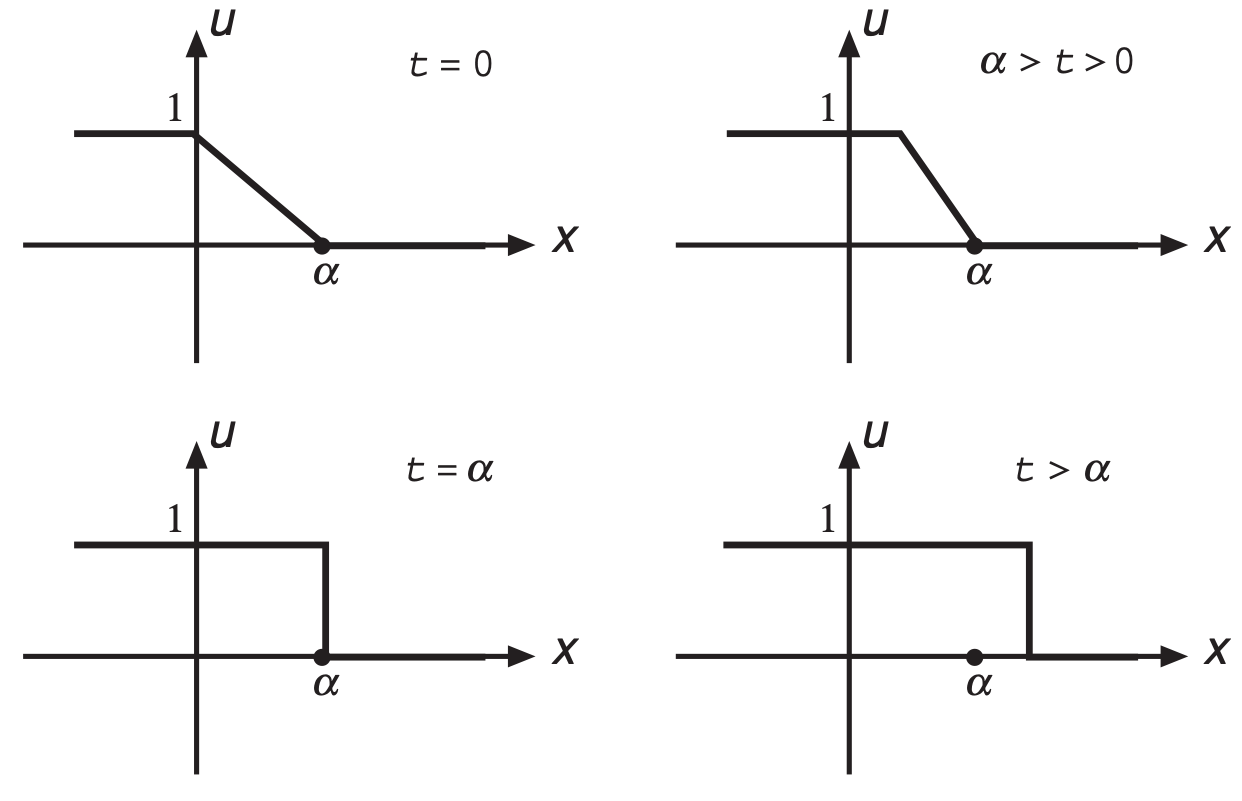
\includegraphics[width=1\linewidth]{img/shock.png}
\captionof{figure}{Several snapshots in the development of a shock wave.}
\end{minipage}

\subsubsection{Entropy Condition}
Characteristics must enter the shock curve, and are not allowed to emanate from it.
\begin{align*}
  F_u(u^-) > \gamma_y > F_u(u^+)
\end{align*}

Applying this rule to the special case $F(u)=\frac{1}{2}u^2$ we obtain that the shock solution is valid only if $u^- > u^+$.
\\
\subsubsection{Case shock wave: $u^- > u^+$} 
The characteristics intersect and it results in a shock wave. The shock wave $\gamma(y)$ describes the curve along which $u(x,y)$ assumes different values. $\gamma_y(y)$ descirbes the speed at which the discontinuity is moving.  The schock wave is given by
\begin{align*}
  u(x,y) &= \begin{cases} u^- & x < \gamma(y) \\ u^+ & x > \gamma(y) \end{cases} &
  \gamma_y(y) &= \frac{F(u^+) - F(u^-)}{u^+-u^-} &
  &\begin{cases} \gamma(y) = \int \gamma_y(y)dy \\ \gamma(0) = \alpha \end{cases} \\
  u^+(y) &= \lim_{x \to \gamma_y(y)_+} u(x,y) & u^-(y) &= \lim_{x \to \gamma_y(y)_-} u(x,y)
\end{align*}
$\alpha$ is the projection of the discontinuity point of the shock wave to $y = 0$.

$y_c$ denotes the critical time where the solution becomes non-smooth. That is, the classical solution is not well defined for $y>y_c$.
\begin{align*}
  y_c &= \inf_{s \in \mathbb{R}} \left\{ -\frac{1}{h'(s)} : h'(s) < 0 \right\} &
  h(s) &= u(x,0)
\end{align*}
If $h(s)$ (the initial value) has a discontinuity (e.g. a step), $y_c = 0$: the solution is weak immediately.
% \subsubsection{Case dilution wave: $u^- < u^+$} 


\clearpage

% You can even have references
\rule{0.3\linewidth}{0.25pt}
%\scriptsize
%\bibliographystyle{abstract}
%\bibliography{refFile}
\end{multicols}
\end{document}
